\documentclass{article}

\usepackage{comment}
\usepackage[english]{isodate}
\usepackage{graphicx}
\usepackage[margin=1in]{geometry}
\usepackage{ragged2e}
\usepackage{wrapfig}

\usepackage{listings}
\usepackage{siunitx}
\usepackage{paracol}
\usepackage{amsmath}
\usepackage{bbm} %mathbb for digits
\usepackage{ amssymb }
\usepackage[utf8]{inputenc}
\usepackage[T1]{fontenc}
\usepackage[bookmarks=true]{hyperref}
\usepackage{bookmark}
\usepackage{pdfpages} %\includepdf[pages={1}]{myfile.pdf}


\usepackage{mathtools,xparse}

\DeclarePairedDelimiter{\abs}{\lvert}{\rvert}
\DeclarePairedDelimiter{\norm}{\lVert}{\rVert}

\newcommand{\E}{\mathbb{E}}
\newcommand{\Var}{\mathrm{Var}}
\newcommand{\Cov}{\mathrm{Cov}}
\newcommand{\iidS}{\overset{iid}{\sim}}
\newcommand{\dS}{\mathcal{S}_k}
\DeclareMathOperator*{\argmax}{arg\,max}
\DeclareMathOperator*{\argmin}{arg\,min}

\sisetup{output-decimal-marker = {,}}
\newcommand*{\ft}[1]{_\mathrm{#1}} 
\newcommand*{\dd}{\mathop{}\!\mathrm{d}}
\newcommand*{\tran}{^{\mkern-1.5mu\mathsf{T}}}%transpose of matrix
\newcommand{\trace}{\mathrm{trace}}

%%new
\newcommand{\tab}{\hspace{.2\textwidth}}
%\newcommand{\span}{\mathrm{Span}}
\renewcommand{\baselinestretch}{1.5}



%%%indenting
\newlength\tindent
\setlength{\tindent}{\parindent}
\setlength{\parindent}{0pt}
\renewcommand{\indent}{\hspace*{\tindent}}


\begin{document}
\begin{titlepage}
\begin{center}
\vspace*{1cm}
\textbf{IFT6269-A2018}\\
\text{Probabilistic Graphical Models}\\
\vspace{0.5cm}
Assignment I

\vspace{1.5cm}

\textbf{Frédéric Boileau}\\
\textbf{p0991440}\\
\vspace{2cm}
Prof. 
Simon Lacoste-Julien
\vfill
\today
\thispagestyle{empty}
\end{center}
\end{titlepage}
\clearpage

\newcommand{\No}{\mathcal{N}}
\graphicspath{{figures/}}

\tableofcontents
\newpage


\section{Generative Model and Theoretical Results}
$Y \sim \mathrm{Bernouilli}(\pi), \quad X\vert Y = j \sim \mathcal N (\mu_j,
\Sigma)$\\[1ex] First let us write the two joint distributions implied by the
definition:
\begin{align*}
    P(x_i, Y = 1) &= P(x_i \vert Y = 1)P(Y=1) = \pi\No(x_i \vert \mu_1, \Sigma)\\
    P(x_i ,Y = 0) &= P(x_i \vert Y = 0)P(Y=0) = (1-\pi) \No (x_i \vert \mu_2, \Sigma)
\end{align*}
Now taking the product of the observations for the likelihood function we have:
\begin{equation}
    L(\theta) =  P(X, Y \vert \mu, \Sigma , \pi) = \prod_{i=1}^{N}
    	\{\pi\No (x_i \vert \mu_1, \Sigma)\}^{y_i}
	\{(1-\pi)\No (x_i \vert \mu_2, \Sigma)\}^{1-y_i}
\end{equation}
Where $\theta$ is just a surrogate for all the parameters to ease notation.\\
Taking the log we get the log-likelihood function and keeping only the terms 
that depend on $\pi$:
\begin{equation}
l_\pi (\theta) = \sum_{i=1}^{N}\{y_i\ln \pi + (1-y_i)\ln (1-\pi) \}
\end{equation}
To maximize we simply take the derivative and set to zero:
\begin{equation}
l_\pi ' = \sum_{i=1}^{N}\left \{\frac{y_i}{\pi}  - \frac{1-y_i}{1-\pi}\right \}  = 0
\end{equation}
Whence we get that 
\begin{equation}
\pi_{MLE} = \frac{1}{N}\sum_{y=1}^N = \frac{N_1}{N_1 + N_2}
\end{equation}
Where $N_1 = \vert \{i : y_i = 1\}\vert$ and $N_2 = \vert \{i : y_i = 1\}\vert$\\
Now for $\mu_1$:
\begin{equation}
    l_{\mu_1} = -\frac{1}{2}\sum_{i=1}^N y_i (x_i - \mu_1)\tran \Sigma^{-1}(x_i
    - \mu_1) + const 
\end{equation}
%
Taking the derivative and setting to zero :
\begin{align*}
    l_{\mu_1}' &= -\frac{1}{2} \sum_{i=1}^N y_i (x_i-\mu_1)\tran(\Lambda + \Lambda\tran)\\
    \intertext{Where $\Lambda = \Sigma^{-1}$ is the precision matrix which is symmetric
    as well :}
    0 &= \sum_{i=1}^N y_i (x_i-\mu_1)\tran \Lambda 
        =\sum_{i=1}^N y_i (x_i-\mu_1)
\end{align*}
All in all we have that 
\begin{equation}
    \mu_{1_{MLE}} = \frac{1}{N_1}\sum_{i=1}^N y_i x_i \qquad 
    \mu_{2_{MLE}} = \frac{1}{N_2}\sum_{i=1}^N (1-y_i) x_i
\end{equation}
%
Where the latter is obtained
following the same steps for $\mu_2$ but replacing $y_i$ by $1-y_i$.
Indeed, in general,  if we have some vector of
mixture proportions $\alpha$ whose components sum to 1 the MLE for the respective means
would be the weighted sum of the observed $x_i$ divided by the number of data points in
the corresponding classes.\\
\clearpage
For the MLE estimate of the covariance matrix we consider the relevant
terms of the "sum expansion" of the log-likelihood which gives:
\begin{equation}
    l_{\Sigma}(\theta) = \frac{N}{2} \log \abs {\Sigma^{-1}}
			-\frac{1}{2} \sum_I y_i (x_i - \mu_1)\tran 
			    \Sigma^{-1}(x_i - \mu_1)
			 -\frac{1}{2} \sum_I (1-y_i)(x_i - \mu_2)\tran 
			    \Sigma^{-1} (x_i - \mu_2) 
\end{equation}

Taking the derivative with respect to $\Sigma$:

\begin{align*}
D_{\Sigma^{-1}}l_{\Sigma}(\theta) = 
  &\frac{N}{2}  \Sigma
  -\frac{1}{2} \sum_I y_i \frac{\partial}{\partial \Sigma^{-1}}
      tr[(x_i - \mu_1)\tran \Sigma^{-1}(x_i - \mu_1)]
      -\frac{1}{2} \sum_I (1-y_i) \frac{\partial}{\partial \Sigma^{-1}}
      tr[(x_i - \mu_2)\tran \Sigma^{-1} (x_i - \mu_2)] \\[1ex]
%
  = & \frac{N}{2} \Sigma
    -\frac{1}{2} \sum_I y_i \frac{\partial}{\partial \Sigma^{-1}}
	  tr[(x_i - \mu_1)(x_i - \mu_1)\tran \Sigma^{-1}]
      -\frac{1}{2} \sum_I (1-y_i) \frac{\partial}{\partial \Sigma^{-1}}
      tr[(x_i - \mu_2)(x_i - \mu_2)\tran \Sigma^{-1} ] \\[1ex]
%
  = & \frac{N}{2} \Sigma
    -\frac{1}{2} \sum_I y_i  (x_i - \mu_1)(x_i - \mu_1)\tran 
      -\frac{1}{2} \sum_I (1-y_i) (x_i - \mu_2)(x_i - \mu_2)\tran  \\[1ex]
\end{align*}
Finally setting to zero we have:
\begin{equation}
    \Sigma = \frac{1}{N}[ \sum_I y_i  (x_i - \mu_1)(x_i - \mu_1)\tran +
    \sum_I (1-y_i) (x_i - \mu_2)(x_i - \mu_2)\tran]  
\end{equation}
\textit{Note on notation}: We have used subscript in $x_i$ as indicating the ith sample
of the random variable and not its ith component.\\
\clearpage

b) Let $\pi = \pi_1$ and $1-\pi = \pi_2$ for notational convenience. Moreover
let the events $Y=1$ and $Y=0$ be denoted $C_1$ and $C_2$ respectively for the
same reason.\\
By Baye's theorem we have:
\begin{align}
    p(C_1 \vert x) &= \frac{p(x\vert C_1)P(C_1)}{p(x\vert C_1)P(C_1) +
    p(x\vert C_2)P(C_2)}\\[2ex]
		   &= \frac{\pi_1 \No (\mu_1, \Sigma) }{\pi_1 \No (\mu_1, \Sigma) 
			    +\pi_2 \No (\mu_2, \Sigma) }
\end{align}
Now letting $ \alpha \triangleq \log \frac{\pi_1 \No (\mu_1, \Sigma)}{\pi_2 \No
(\mu_2, \Sigma) }$ we have that :
\begin{equation}
p(C_1 \vert x) = \frac{1}{1+\exp(-\alpha)} \triangleq \sigma (\alpha)
\end{equation}
Now let us examine the expression "$\alpha$", the argument to the logit function
in this form.
\begin{align*}
    \alpha &= \log\left[\frac{p(x\vert C_1)p(C_1)}{p(x\vert C_2)p(C_2)}\right]\\[1ex]
	 &= \log\left[\frac{\pi_1 \exp(-1/2(x-\mu_1)\tran \Sigma^{-1} (x-\mu_1))}
			 {\pi_2 \exp(-1/2(x-\mu_2)\tran \Sigma^{-1} (x-\mu_2))}
	     \right] \\[1ex]
	 &= \log\left(\frac{\pi_1}{\pi_2}\right)
	    - 1/2(x-\mu_1)\tran \Sigma^{-1} (x-\mu_1)
	    + 1/2(x-\mu_2)\tran \Sigma^{-1} (x-\mu_2)
	 \intertext{And the quadratic terms cancel out so that:}
	 &= \frac{1}{2}x\tran \Sigma^{-1}\mu_1 
	    -\frac{1}{2}x\tran\Sigma^{-1}\mu_2
	    -\frac{1}{2}\mu_1\tran\Sigma^{-1}\mu_1 
	    +\frac{1}{2}\mu_2\tran\Sigma^{-1}\mu_2
	    +\log\left(\frac{\pi_1}{\pi_2}\right) 
\end{align*}
Now defining the following parameters:
\begin{equation}
	w = \Sigma^{-1}(\mu_1 - \mu_2) \qquad
	w_0 = -\frac{1}{2}\mu_1\tran\Sigma^{-1}\mu_1 
	+\frac{1}{2}\mu_2\tran\Sigma^{-1}\mu_2
	 + \log\left(\frac{\pi_1}{\pi_2}\right) 
\end{equation}
We get that the class conditionnal can be expressed as the result of applying the
logit function to an affine transformation in $x$:
\begin{equation}
	P(C_1\vert x) = \sigma(w\tran x + w_0)
\end{equation}
We can see that the last term in $w_0$ is the $\log$ of the ratio of the priors
on the classes. We can thus see that under the current assumptions on the distribution
of $X \vert C_k \sim \No (\mu_k, \Sigma)$ changing the priors will only offset the decision
boundaries.
Clearly for $P(C_1\vert x) = \sigma(f(.))$ to be equal to a constant we need the 
function $f(.)$ to be constant too. Moreover $\sigma(c) = 0.5$ implies 
that $c$ equals zero. Therefore the decision boundary is the solution to
the affine equation $w\tran x + w_0 = 0$. The linearity is the result of
enforcing both class conditionnals to share the same covariance matrix, 
removing this assumption would result in quadratic boundaries.\\
So there many similarities between our model and the logistic regression,
including a linear decision boundary hence they are both "linear".
However we are dealing with a generative model and the parameters 
to the affine map were determined by finding the MLE of the underlying
distributions of $X \vert C_k$ which were "known". 
In logistic regression the parameters $w$ and $w_0$ to the affine map
are in themselves computed by MLE. 
\clearpage

\section{Experimental Results}
\subsection{Generative Model}
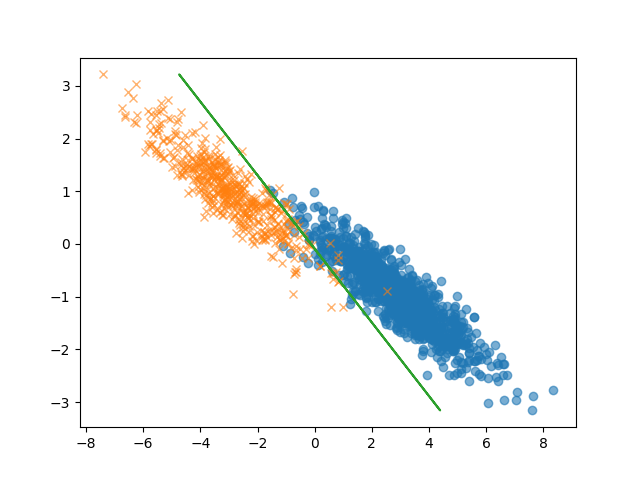
\includegraphics[height= 0.3\textheight]{generativeFig0.png}
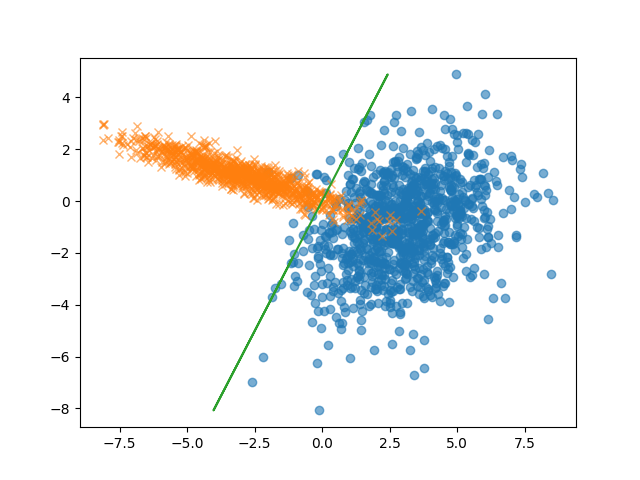
\includegraphics[height= 0.3\textheight]{generativeFig1.png}
\begin{center}
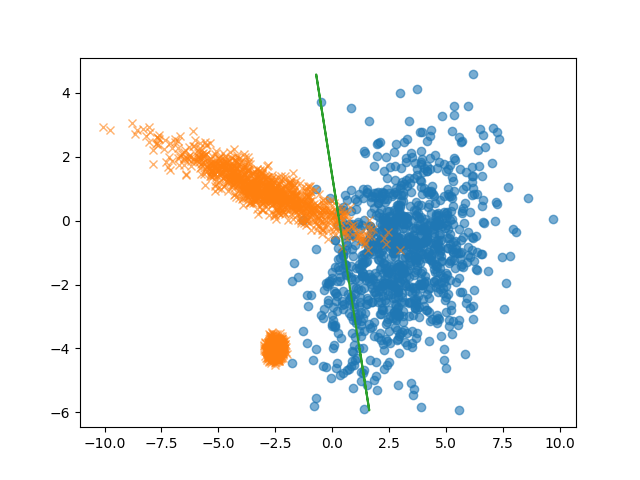
\includegraphics[height= 0.3\textheight]{generativeFig2.png}
\end{center}
\begin{align*}
  \Sigma_A  = \begin{bmatrix} 4.12 & -1.66\\ -1.66 &  0.783 \end{bmatrix} \qquad
  \Sigma_B  = \begin{bmatrix} 6.05 & -0.921\\ -0.921 & 1.98 \end{bmatrix} \qquad
  \Sigma_C  = \begin{bmatrix} 4.79  & -0.734\\ -0.734 &  5.39 \end{bmatrix}
\end{align*}

\begin{alignat*}{3}
    \mu_{A1} &=  [ -0.879, 0.281 ]
    \qquad &\mu_{A2} &=  [ 1.95, -0.600 ]\\
    \mu_{B1} &= [ -1.60, 0.542 ]
    \qquad &\mu_{B2} &= [ 1.68, -0.419 ]\\
    \mu_{C1} &=  [ -1.84, -0.603 ]
    \qquad &\mu_{C2} &= [ 1.05, -0.315 ]\\
\end{alignat*}
\clearpage

%
\subsection{Logistic Regression}
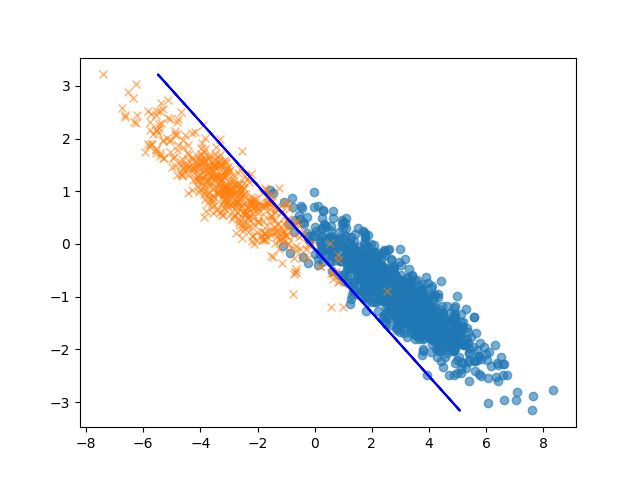
\includegraphics[height= 0.3\textheight]{logisticRegression0.png}
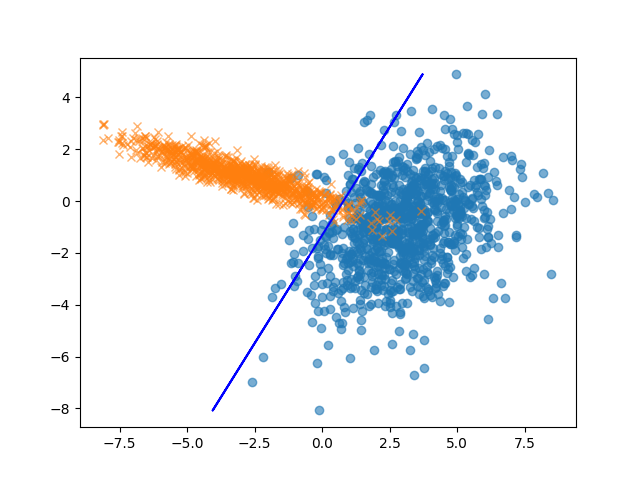
\includegraphics[height= 0.3\textheight]{logisticRegression1.png}
\begin{center}
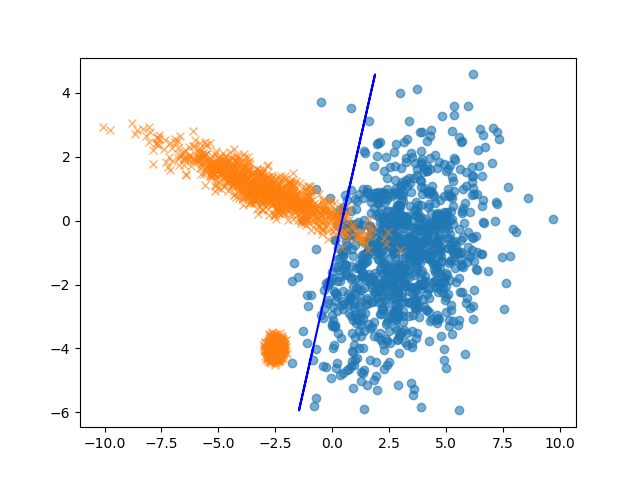
\includegraphics[height= 0.3\textheight]{logisticRegression2.png}
\end{center}

\begin{equation}
  w_1 = [ -1.22, -7.79, -12.9] \qquad 
  w_2 = [ 1.32, -1.68, 1.01] \qquad
  w_3 = [ 0.940 -2.18  0.692]
\end{equation}
\clearpage
% 
\subsection{Linear Regression}
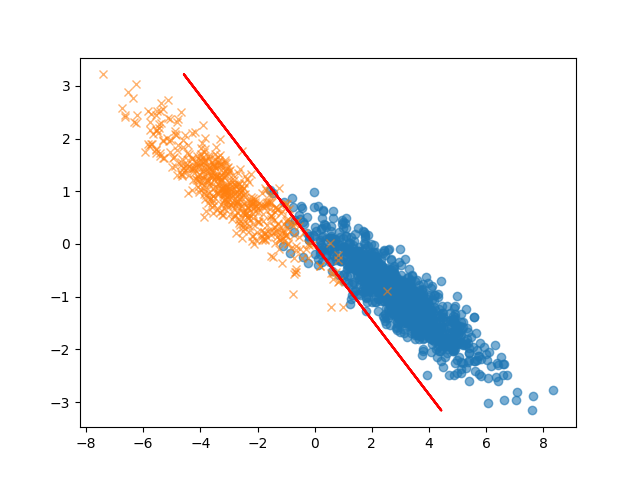
\includegraphics[height= 0.3\textheight]{LinearRegression0.png}
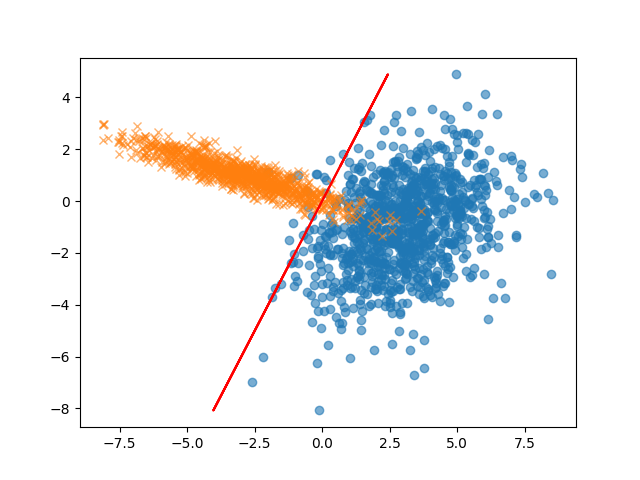
\includegraphics[height= 0.3\textheight]{LinearRegression1.png}
\begin{center}
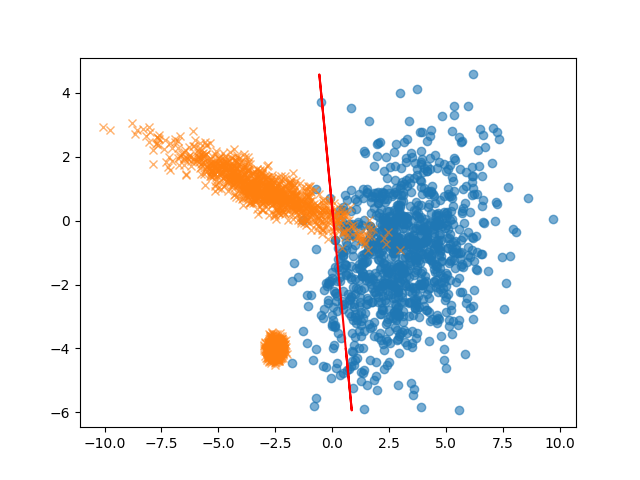
\includegraphics[height= 0.3\textheight]{LinearRegression2.png}
\end{center}

\begin{equation}
w_1 = [ 0.492, -0.264, -0.373] \qquad
w_2 = [ 0.499, -0.104,  0.0519] \qquad
w_3 = [ 0.507, -0.128, -0.0173]
\end{equation}
\clearpage

\subsection{QDA}
\clearpage

\subsection{Comparison and Discussion of Models}
\begin{figure}[htbp!]
\begin{center}
\begin{tabular}{| c | c | c | c |}
\hline
&A & B & C\\
\hline
Linear Generative Model &0.00800& 0.00900 & 0.0370\\
\hline
Logistic Regression & 0.0113 &  0.0270 & 0.00900\\
\hline
Linear Regression & 0.0133 & 0.00900 & 0.0207\\
\hline
QDA & . & . &\\
\hline
\end{tabular}
\end{center}
\end{figure}

\clearpage
\section{Code}








\end{document}
